%!TEX root = project.tex
\begin{titlepage}
   \begin{center}
       \vspace*{1cm}

       \textbf{Acknowledgements}
       \end{center}
       We would like to take this part of the dissertation to acknowledge our supervisor Martin Kenirons and the GMIT staff for all of their support and help throughout our final year project and over the past four years.
\end{titlepage}

\chapter*{About this project}
\paragraph{Abstract}
People often buy items that they only intend to use once, and just throw it in the corner for eternity. Even aside from the one-off purchases, many of people's belongings are barely used by them and are left idle for most of the time. BarterNearMe is a website which offers a solution to this problem in the form of a 21st century barter system. This website provides users with the ability to login, register and browse or add available items and wanted items. The user may also save an available item for later viewing. 

\paragraph{Authors}
Explain here who the authors are. Nathan Garrihy and Cathal Donohoe.



\chapter{Introduction}

% The introduction should be about three to five pages long. (5 recommended)
% Provide a clear context for your project.
% – What is it about? Is it at the right level (8)?
% – Is the scope correct?
% – Do not assume that the reader knows anything about the domain.
% – Why should a reader care or be interested?
% q Set out the objectives of the project clearly.
% – You will have to address each of these in the evaluation /
% conclusion.
% – The metrics by which success or failure is measured.
% q Briefly list each chapter / section and provide a brief description
% of what each section contains.
% – List the resource URL (GitHub address) for the project and provide
% a brief list and description of the main elements at the URL.
% q After reading the introduction, a reader should be 100% certain
% of what the project is all about and why it is relevant.
% Make sure you use references~\cite{einstein}

At the beginning of our final year, our year were given the opportunity to work as a team or individually to develop a project over the course of the year across two semesters. We worked together on the end of year project in year 3 semester 6 of the course in which we developed a first person shooter in Unity. We were both very happy with our results and our ability to work together so we decided to group up together along with a fellow student Anton Golubev. We knew that what we were to develop had to be up to standards for a level 8 final year project, had to use a multitude of languages, technologies and had to test our knowledge and kills to improve them as software developers. Our initial ideas mostly centered around a CRUD(Create-Read-Update-Delete) application focused on E-commerce or a social media platform. After much debate as to what our final year project would consist of, we agreed on an E-commerce website in users could upload, view and save products for buying and trading. The intention of the project was to improve our abilities and understanding of new technologies and create a better foundation of our skills in our field of work.

\section{The Idea}
Our final decision on an idea for the final year project was to develop a full stack CRUD application developed for trade and exchange of items between multiple users. The website is quite similar in style to DoneDeal, except our site promotes users to get in contact with each other to trade items with one another for a period which they see as appropriate.

\section{Scope}
%Project scope is a detailed outline of all aspects of a project, including all related activities, %resources, timelines, and deliveries, as well as the project's boundaries. 
%Who, What, When, Where, Why
We both grew up in a close-knit community surrounded by friendly neighbours and oftentimes if our family required something like a ladder, or a drill for the day, our neighbours would allow us to borrow one for as long as necessary. After moving to Galway for college, we noticed that cities really lack that close-knit connection as many people don't even know their neighbours well enough to ask to borrow an item. This got us thinking and our solution was a website designed so that users can browse items and acquire contact details for the owner of the listed item, if desired. This website is a useful way of saving money by offering the ability to temporarily acquire items which are only required once. \newline
The initial scope intended for this project to be completed by 3 students. However, we were struck with a slight roadblock as we had to re-define the scope in December as one of our team members was unable to continue with 4th Year due to personal reasons inflicted by the COVID-19 pandemic.

\subsection{Objectives}
Targets we hoped to achieve with this project. The main functionality we wanted to achieve was:
\begin{itemize}
    \item Users can register and browse items

    \item Users can select to borrow items from other users

    \item Users can view the owners of items and contact them

    \item Users can add items to a Wishlist
\end{itemize}
We aimed for the website to allow users to register or login using an email and password which is stored in a database. We aimed to allow users to post items they want to borrow as well as items they have which they can loan out to a database and display these items on the website for all users to view. We were unsure about how we could allow users to contact owners of other items, but we wanted to leave it mostly the users responsibility to organise the borrowing of items since handling it ourselves could potentially lead to legal implications. i.e. if somebody gets robbed, we should not be held accountable.

\subsubsection{Timelines}
Upon starting the project, we aimed to have a working prototype with a login and sign up working to show for the presentation in late December. However, the loss of a team member on the run up to Christmas meant that we had to re-scope the project, scaling it down so that we would be finished with it by the due date in May. This delay made us unable to merge the working front end with the working back end code and we had to show the 2 separate prototypes for the presentation.
We also set some milestones around this time which we used along with the guidance of our supervisor to ensure we didn't fall behind. These were:
\begin{itemize}
    \item January 31st - Get react and spring boot working together (talking).

    \item February 28th - Users can add+view items for trade

    \item March 31st - User can add+view wanted items

    \item April 15th - Users can save ads to their saved-items for later
    
    \item April 30th - All unimplemented features added to the site, dissertation complete
    
    \item May 7th - All testing and bug fixes complete
\end{itemize}

\subsection{Deliverables}
 Deliverables we need to produce in order to meet all requirements. 
 
\subsubsection{Application}
\begin{itemize}
\item A link to \underline{\href{https://github.com/CathalDonohoe/FinalYearProject}{the GitHub repository}} containing the full source code for the website.
\item A working version of the website deployed to AWS.
\end{itemize}

\subsubsection{Documentation}
\begin{itemize}
\item A PDF file containing this dissertation
\item This dissertation in latex format
\item README file with instructions of how to interact with the website
\item A brief screencast of the working application
\end{itemize}
 
\subsection{Boundaries}
The main things that were left out in this project were left out because of the loss of a group member. We had planned to do a review system where the borrower and lender provide each other with a small review and rating out of 10 after completing a transaction to show that those users are trustworthy. This would have been a nice feature as it's hard to trust anyone these days. However, we decided not to implement this feature when we scaled the project back a bit in December.  

\section{Overview of chapters}
This dissertation is divided into chapters, each of which contains information about a different aspect of the project. We'll list these chapters and provide a brief summary of each in this section. 

\subsection{Methodology}
The methods we used to build our project will be described in this section. The approach would delve into the basic processes and strategies used by the project at hand. It will describe our development process, as well as version control and testing.  

\subsection{Technology Review}
This section will cover the technologies we discovered and used during our research and development. Different technologies, such as Spring Boot, React, MongoDB, and AWS, will be plotted and evaluated. We'll go into how to set them up and how to use them. 

\subsection{System Design}
This chapter provides an overview of how the whole system architecture is designed and how it all works together, with diagrams to help explain each component of the system. 

\subsection{System Evaluation}
The performance, robustness, and scalability of the system will be discussed in this section of the dissertation. We'll also go through the benefits and drawbacks we faced while working on this project. 

\subsection{Conclusion}
The conclusion is a segment in which we summarize our observations, conclusions, and insights gained while developing and deploying this project. 

\section{GitHub Info}
The project can be found on \underline{\href{https://github.com/CathalDonohoe/FinalYearProject}{this GitHub repository}}, located at \url{https://github.com/CathalDonohoe/FinalYearProject}

\chapter{Methodology}
Methodology is the study of methods used in a field. Its the collection of methods, practices, procedures and rules used by those who work in a field of study. This chapter of the dissertation will explain the methods that we used to develop our web application, we will explain the type of development approach that we took to the project, we will explain our validation and testing and lastly we will list and give a small explanation of the technologies that we used in our development process.

\section{Approach to Development}
During the early stages of the project, our supervisor suggested that we split our selves between Back End Development and Front End Development. After a short while of debating where we should dedicate ourselves to on the Development front, we decided that Nathan should focus on Front End Development, as he is especially talented in making GUIs aesthetically pleasing, that Cathal should focus on Back End Development, as he has pass experiences with working with Databases, and that Anton should lend a hand to both sides as he had experience with both ends.\par
After these decisions we decided we should utilize an incremental and iterative approach to development. Since there was three of us working on the project, we found that this approach worked well because we were all operating on different schedules due to the personal reasons, so this development strategy allowed us to have more flexible schedules and relieved a lot of pressure, which was essential considering the pressure we were already under due to the COVID 19 pandemic. \par
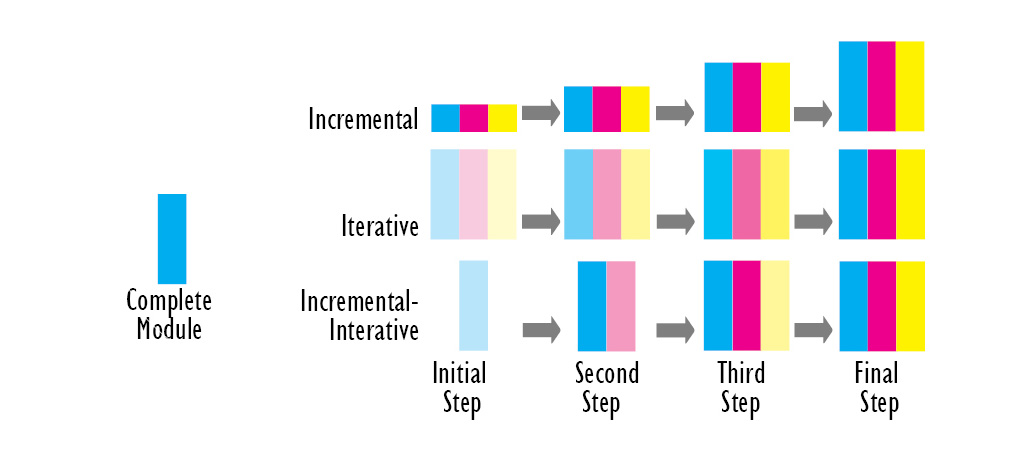
\includegraphics[scale=1.3]{img/Incremental-Interative-Design-Approach.jpg} \newline
\par Iterative and Incremental development is a process that combines the iterative design method with the incremental build model. The combination is of long standing  and has been widely suggested for large development efforts. This Agile method approach to Software Development is modeled around gradually increasing the features of a program and a cyclical release and upgrade pattern. The process usually begins with planning and continues through iterative cycles and the addition of features finishing with the development of a completed program of application at the end of each of these iterative cycles. Below we'll explain each of these individually:
\begin{itemize}
    \item Iterative: The incremental method divides the software development process into tiny, manageable chunks called increments.Each increment builds on the previous edition, allowing for gradual progress. 
    \item Incremental: Iterative software development refers to the process of repeating software development tasks in loops known as iterations. For each iteration, a new version of the program is created before the best product is found. 
\end{itemize}

\section{Validation testing}
This part of the methodology will be dedicated to the Validation testing of our project. This is the method of testing software during the development process or at the end of the development process to see whether it meets those specifications. \par
Validation testing guarantees that the product meets the client's, or in our case, our project's, requirements. It can also be described as demonstrating that the product performs as expected when used in the designated environment. In short it is designed to answer if the product meets the requirements specified.\par
Testing is an integral aspect of a software project's life cycle, and it contributes to the overall consistency and reliability of the code in the project. 

TO BE CONCLUDED- Cathal

\section{Use of GitHub}
GitHub was essential to us during the development phase of the project. The use of GitHub in our development not only allowed us to save and exchange code with ease, but it can also double as a version control manager. We had all used GitHub for personal and academic projects, so we were all very familiar with the hosting service already. 
\section{Criteria}
\subsection{React}
React is an open-source, front end, JavaScript library for building user interfaces or UI components. It is maintained by Facebook and a community of individual developers and companies. We decided to use this for our Front End as it aesthetically pleasing and once saved, the page will update automatically allowing for a quicker and easier development process.

\subsection{Node js}
\cite{NodsJS}Node JS is an asynchronous event-driven platform built on Chrome's JavaScript runtime that allows easy building of efficient, scalable network applications. NPM, or Node Package Manager is the Node JavaScript platform's package manager. It puts modules in place so that node can find themand intelligently manages dependency conflicts. Hundreds of thousands of JavaScript developers use it every day because it's battle-tested and remarkably versatile.

\subsection{Express}
\cite{ExpressJS}Express is a Node.js web application framework that offers a comprehensive set of features for web applications. Express adds a thin layer of basic web application functionality without masking any of Node JS's known features. When utilized correctly, express offers data to be fetched from the server and displayed to the client with ease and offers high scalability as well as exemplary security. It is well constructed and documented, making implementation quite an easy and fast process.

\subsection{Java}
Java is a class-based, object-orientated programming language that is designed to have as few implementation dependencies as possible. This is the language that our Back End API, wrote in the Spring Boot framework, relies on. As we chose our API framework in Spring Boot first, we subsequently had to develop it in in Java. This language is one that Cathal has been programming for 6 years in, so as he focused on the Back End Development this was an ideal language to choose.

\subsection{Spring Boot}
Spring Boot is an open Source Java-Based framework used to create a micro Service. We used this framework to create and store collections in our Mongo Database. Spring Boot is developed by the team at Pivotal, it was designed to simplify the development of a new Spring application. The framework takes an opinionated approach to configuration, freeing developers from the need to define boilerplate configuration. Spring boot provides a good platform for Java developers to develop a stand-alone and production-grade spring application.

\subsection{MongoDB}
MongoDB is a document database, which means it stores data in JSON-like documents. When it came to a decision as to what to use for our database, we had two main choices, MySQL and MongoDB. We both had more experience with MySQL and decided to use a Mongo Database instead to expand our knowledge and experience with more types of technologies.

\subsection{Docker}
Docker is a tool designed to make it easier to create, deploy, and run applications by using containers. Containers allow the developer to package up an application with all of the parts it needs, such as libraries and other dependencies, and deploy it as one package. This was an ideal platform to store our Mongo Database on, and to package our Front End and Back End for deployment on AWS.

\subsection{Robo 3T}
Robo 3T (formerly Robomongo) is a graphical user interface (GUI) for MongoDB hosting deployments that allows users to interact with their data through visual indicators instead of a text-based interface. We decided on using this ton confirm objects being added to our collections as we found the visual indicator to be very pleasing when in comparison to a Command line interface that we would normally use when deploying to a Mongo Database.

\subsection{Postman}
Postman is an API client that makes it east for developers to create, share, test and document APIs. This is done by allowing users to create and save complex HTTP/s requests, as well as read their responses. This allows users to automate manual tests and integrate them into their CI/CD pipeline to ensure that ant code changes wont break the API in production. \par
This allowed us to test our Back End development was working and could POST and GET API calls without a Front End Environment being connected.

\subsection{AWS}
Amazon Web Services (AWS) is a secure cloud service platform, offering compute power, database storage, content delivery and other functionality to help businesses scale and grow. In short, AWS allows the user to run a web application server in the cloud. This is the technology that we decided best suited our needs for deploying the application onto a live server.

\subsection{IntelliJ}
IntelliJ IDEA is an integrated development environment written in Java for developing computer software. It is developed by JetBrains, and is available as a community licensed edition and as a commercial edition. This is the IDE we chose for developing our Java code as it is a visually pleasing and organised IDE. Most of our Java modules required us to use Eclipse, so this was also a nice method of keeping our Final Year Project separate form our other Java code.

\subsection{Visual Studio Code}
Visual Studio Code is a freeware source-code editor made by Microsoft for Windows, Linux and mac OS. it has supported features for debugging, syntax highlighting, intelligent code completion, snippets, code refactoring and embedded GIT. This IDE is ideal for development of JavaScript as it provides a clear and concise UI for the developer.

\subsection{GitHub}
GitHub Inc is a provider of internet hosting for software development and version control using Git. It offers the distributed version control and source code management functionality of git plus its own features. We have been using this platform to store our projects since second year of college, so it was an ideal platform to use again to ensure we both had to most up to date version of our code.

\subsection{Jira}
Jira is a proprietary issue tracking product developed by Atlassian that allows bug tracking and agile project management. This software allows users to create weekly sprints with goals and deadlines to be achieved. We found this to be an ideal methodology for keeping us both knowledgeable of what is to be accomplished next and what needs to be completed.

\subsection{Discord}
Discord is a VoIP, instant messaging and digital distribution platform designed for creating communities. Users communicate with voice calls, video calls, text messaging, media and files in private chats. We used this platform to communicate live when we were both in development. We also used it to exchange texts, code and images with each other through a Discord Server we created.

\subsection{Facebook Messenger}
Facebook Messenger is an American messaging app and platform developed by Facebook inc. This is another service that allows for instant massaging between users. This was our main source of communicating with each other for organisation as it has been our main form of communicating since we were in first year.

\subsection{Microsoft Teams}
Microsoft Teams is a proprietary business communication platform developed by Microsoft. Teams offers work space chat and videoconferencing, file storage and application integration. When Covid-19 first affected us, GMIT switched to using Microsoft Teams for their main form of lecturing and live meetings. We used this platform weekly t have meeting with our supervisor and to communicate with them for advice.

% Check out the nice graphs in Figure \ref{tikz:graphs}, and the nice diagram in Figure \ref{tikz:mydiagram}.

% \begin{figure}
%   \centering
%   \begin{tikzpicture}
%   \begin{scope}[every node/.style={circle,thick,draw}]
%   \node (a) at (0,2) {a};
%   \node (b) at (2,2) {b};
%   \node (c) at (2,0) {c};
%   \node (d) at (0,0) {d};
%   \end{scope}
%   \begin{scope}[every edge/.style={draw=black,thick}]
%   \path (a) edge (b);
%   \path (b) edge (c);
%   \path (b) edge (d);
%   \path (c) edge (d);
%   \end{scope}
%   \node () at (1,-1) {$G_1$};
%   \end{tikzpicture}
%   \hspace{1.5cm}
%   \begin{tikzpicture}
%   \begin{scope}[every node/.style={circle,thick,draw}]
%   \node (1) at (0,2) {a};
%   \node (2) at (2,2) {b};
%   \node (3) at (2,0) {c};
%   \node (4) at (0,0) {d};
%   \end{scope}
%   \begin{scope}[every edge/.style={draw=black,thick}]
%   \path (1) edge (2);
%   \path (1) edge (3);
%   \path (1) edge (4);
%   \path (3) edge (4);
%   \end{scope}
%   \node () at (1,-1) {$G_2$};
%   \end{tikzpicture}
%   \caption{Nice pictures}
%   \label{tikz:graphs}
% \end{figure}


% \begin{figure}
%   \centering
%   \begin{tikzpicture}[node distance=6cm]
%   \node (a) [rect] {A Big Blue Block};
%   \node (b) [oval, right of=a] {And His Oval Friend};
%   \draw [line] (a) -- (b);
%   \end{tikzpicture}
%   \caption{Nice pictures}
%   \label{tikz:graphs}
% \end{figure}


\chapter{Technology Review}

About seven to ten pages.///////
 When we decided that we would be developing a CRUD application our first step was to decide upon what technologies we would be using to develop and test the application. This section will be split into four main focus points; The technology used in the Front End of the application, the technology used in the Back End of the application, the technology used for development, and the technology that is used to organise the development process of the application.
\begin{itemize}
\item Describe each of the technologies you used at a conceptual level. Standards, Database Model (e.g. MongoDB, CouchDB), XMl, WSDL, JSON, JAXP."break in". The Front End: the technologies that were used in the Front End development were React...
\item Use references (IEEE format, e.g. [1]), Books, Papers, URLs (timestamp) – sources should be authoritative. "break in". The Back End: the technologies that were used in the Back End development were Spring Boot, MongoDB, Docker, Robo 3T, Postman and AWS.
\item This section will cover the technology used for the development process, mainly the Integrated Development Environments, IntelliJ and Visual Studio Code.
\item Lastly is the technology used in the organisation of the project development: Github, Jira, Discord and Microsoft Teams.
\end{itemize}

\section{Front End Technology}
\subsection{React}
The front end for this website was coded up using the React framework. We had only used React once before, in 3rd year, when we created a MERN (MongoDB, Express, React, Node) web application. Although one module during semester wasn't too much time, it was evident during this period that as well as being well documented and relatively user friendly, react is a very advanced framework.
\begin{center}
    
\includegraphics[width = 16cm, height = 8cm]{img/reactImage.jpeg}
\end{center}
    
\subsubsection{Why React?}
There was a wide range of technical problems which was faced in web development. \cite{IntroductionReact}A large number of these problems were solved when Facebook came out with react and it has been constantly improving since its release in May 2013. React was brought out to solve complex user interface problems and utilizes a philosophy first thought up by Eric Raymond in 2003.

\begin{quote}
\cite{ArtOfUnix}\emph{The only way to write complex software that won't fall on its face is to hold global complexity down - to build it out of simple parts connected by well defined interfaces - so that most problems are local and you can have some hope of upgrading a part without braking the whole - Eric S. Raymond}
\end{quote}

\cite{IntroductionReact}React allows data to be displayed on wide scale user interfaces with relative ease. While most frameworks adopt a model, view, controller architecture, it would not be entirely accurate to place React under this category as React focuses more on the "view" as opposed to the model and controller. \newline
React has a range of libraries which can be imported to add functionality to the framework.\cite{Axios} An example of a library which was used is axios, which is a library that aids the sending of http requests to external resources. Axios, as well as many of the other React libraries is well documented and has plenty resources out there to aid development.

\subsection{Nods.js}
We used Node JS because it provides all of the benefits of \cite{fullStackJS}full stack JS development. These include

\begin{itemize}
    \item Improved overall efficiency and productivity
    \item Better speed and performance
    \item Wide range of free tools
\end{itemize}

Due to its asynchronous, single-threaded nature, it works very well with React's responsive web pages and this was very useful during development as it minimised the time to wait between adding a feature and seeing if that feature worked since the website updated in what was pretty much real time. \cite{PaypalNodeJS}Big companies such as PayPal use NodeJS as apposed to something like Java and it's known to allow faster serving of web pages as well as reducing the time it takes to develop server-side software.\newline
Node makes it very easy to handle all the packages that are required to run the application. It performs a lot of processes with efficiency in the background and provides very user friendly error messages whenever any problems arise during the installation of packages or when running the server. Node removes a lot of the heavy work involved in getting a website to function correctly, and it works extremely well when coupled with React.

\subsection{Express}
Express has some \href{https://expressjs.com/en/5x/api.html}{good quality documentation}. And although we only coded a tiny portion of this website using express, it was well documented, making it easy to find what we were looking for and implement it correctly. As express state that they are a \cite{ExpressRM}\emph{"Fast, unopinionated, minimalist web framework for node."} Express provides robust routing, focuses on high performance, has great test coverage, provides HTTP helpers for things like caching and redirection. Express also provides an executable which provides simple and quick generation of applications. 

\subsubsection{express.json} 
Json is a built-in middleware function in Express. Express.json parses requests received with JSON payloads and it is based on body-parser, which parses incoming request bodies in a middleware. 

\subsubsection{express.router}
A router Object behaves like middleware in that its sole purpose is performing routing and middleware functions. The express router offers a wide range of methods which can be used to acquire all sorts of routing functionality that enable the top level express object to essential operate as a router. Express router can be used with Nodemailer to send emails with fast routing.

\subsubsection{Nodemailer}
Nodemailer is a NodeJS module that makes sending emails as quite easy. First released in in 2010, at a time where sending email messages was a difficult task, it has now evolved to be the preferred solution for the majority of NodeJS users.
The Nodemailer team have a strong focus on security and integrity, which was the main reason why we saw it fit to be our email sending module of choice.

\subsection{Other technologies considered}
We also considered Angular for the back end framework since we also used Angular for a semester. However, along with Nathan's personal preference of React, its virtual DOM makes it perform much better than Angular. Also, React is the more popular framework and this wider community means more documentation and more activity on forums such as \underline{\href{https://stackoverflow.com}{StackOverflow}}. React goes well with Spring Boot and MongoDB, which was another leading factor in deciding what back end technology to use.  \newline

\section{Back End Technology}

\subsection{Java}

\includegraphics[scale = 0.6]{img/java-logo-1.png}\newline
The main coding language used on the Back End Development of the project is Java. Java was originally developed by James Gosling at Sun Micro systems (Later to be acquired by Oracle) and released in 1995 as a core component of Sun Micro systems' Java platform. Java is a general-purpose programming language intended to let application developers write once, run anywhere(WORA), meaning that compiled Java code can run on all platforms that support Java without the need of recompilation. \par
This was the main reason in our choosing of the language for an application in which we intended to deploy, allowing us to not have to worry about errors once the program executed locally without any compilation errors. This is also a language in which we both had many years of experience in allowing us to commit the time we had gained by already knowing the language for our development, into other technologies we hadn't used such as AWS or MongoDB.

\subsection{Spring Boot}
Spring Boot Auto Configuration automatically configures the Spring Boot Application based on the JAR dependencies added in the project. For example with this application when we are using the Mongo Database, we don't need to configure a database connection, the Spring Boot auto-configures an in-memory database. To do this though we must add the @EnableAutoConfiguration annotation to the main class file. Then the Spring Boot application will be automatically configured.\par
Spring Boot application scans all the beans and package declarations when the application initializes. the @ComponsnentScan annotation must be added for the class file to scan the components added to the project. \par
The class that contains the @SpringBootApplication and the main method is the entry point of the spring boot application. This class must have the main method to run the Spring Boot applicaton. The @SpringBootApplication annotation includes the Auto-configuration, Component Scan and the Spring Boot Configuaration. Since the @SpringBootApplication annotation has been added to the main class we do not need to add the @EnableAutoConfiguration, @ComponentScan and the @SpringBootConfiguration annotations. The @SpringBootApplication annotation includes all other annotations. \par
See the following code for a better understanding:
\begin{minted}{java}
import org.springframework.boot.SpringApplication;
import org.springframework.boot.autoconfigure.SpringBootApplication;

@SpringBootApplication
public class FyPprojectApplication {

	public static void main(String[] args) {

		SpringApplication.run(FyPprojectApplication.class, args);
	}

}
\end{minted}
Spring Boot's use of these Auto-configuration allowed us to streamline our development of the Back End Environment of the project. Simply by adding dependencies into our pom file of the Spring Boot application, our program will auto-configure it upon compile time. \par
\begin{minted}{java}
<dependency>
	<groupId>org.springframework.boot</groupId>
	<artifactId>spring-boot-starter-data-mongodb</artifactId>
</dependency
\end{minted}

\subsection{MongoDB}

\includegraphics[scale=0.5]{img/MongoDB-logo.png} \newline
MongoDB is the leading modern, general purpose database platform, designed to unleash the power of software and data for developers and the applications they build. Its built upon the document model, a fundamentally different model than traditional relational databases. \par
In real world applications it is common place for the data for a single object, like a patient or a user, to spread out among dozens of tables. This adds a massive amount of complexity to the application. This can add a number of downsides to the application:
\begin{itemize}
\item It can make the maintenance of the application hard to understand
\item Secondly it can make adding features harder as there is more to account for
\item Lastly pulling data from so many areas is inefficient and the applications need to have code to deal with this
\end{itemize}
\par MongoDB takes an entirely different approach, data is stored in records called documents and just like real physical records, documents can house multiple phone numbers, addresses and more and can be right next to another document that only has one address and no phone number. Records aren't restricted to having the same number of columns. These documents allow us to store data in a way that is easy for the computer to process and natural for humans to read. This allowed us to no longer have to make our application to accommodate the needs database, MongoDB accommodates us to allow us to store our data in a more natural way. This allowed us to add new data to each collection without having to worry about breaking previous data. \par

\subsection{Docker}

\includegraphics[scale=0.2]{img/docker-logo.png} \newline
Docker is a Software Development platform with aspects of a virtualisation technology that makes it easy for developers to develop and deploy applications inside neatly packaged virtual container environments. This means that Docker allows applications to run the same no matter where they are or what type of machine they are running on. Docker containers can be deployed to any machine without any compatibility issues so that our software stays system agnostic making the software simpler to use, less work to develop and easy to maintain and deploy. \par
These containers running on the computer or server act as miniature micro heaters, each with their own specific job, operating system,isolated CPU processes, memory and network resources. Because of this these containers can be easily added, removed, stopped and started without affecting the run time machine. Containers usually run one specific task, in our case that is the Mongo Database, the React application and the Spring Boot application. These containers are then networked together and potentially scaled. A developer can access the Docker Hub and pull a pre-configured container designed for a specific task from the Hub and integrate it into their own environment. We deiced to make these containers ourselves to gain a better understanding and knowledge of our containers and to ensure that the containers were not executing any unneeded or redundant features.

\subsection{Robo 3T}
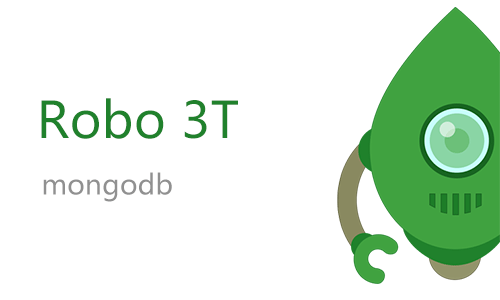
\includegraphics[scale=0.6]{img/robo-logo.png}\newline
Robo 3T is effectively a MongoDB manager. We used Robo 3T to check the Mongo database without having to use a Command Line. This allowed us to visualise our database in a more innovative way. It can be used on multiple OS's including Windows, Linux and MAC. Once Robo 3T has been loaded, it will open up a GUI asking for the user to connect to. \par
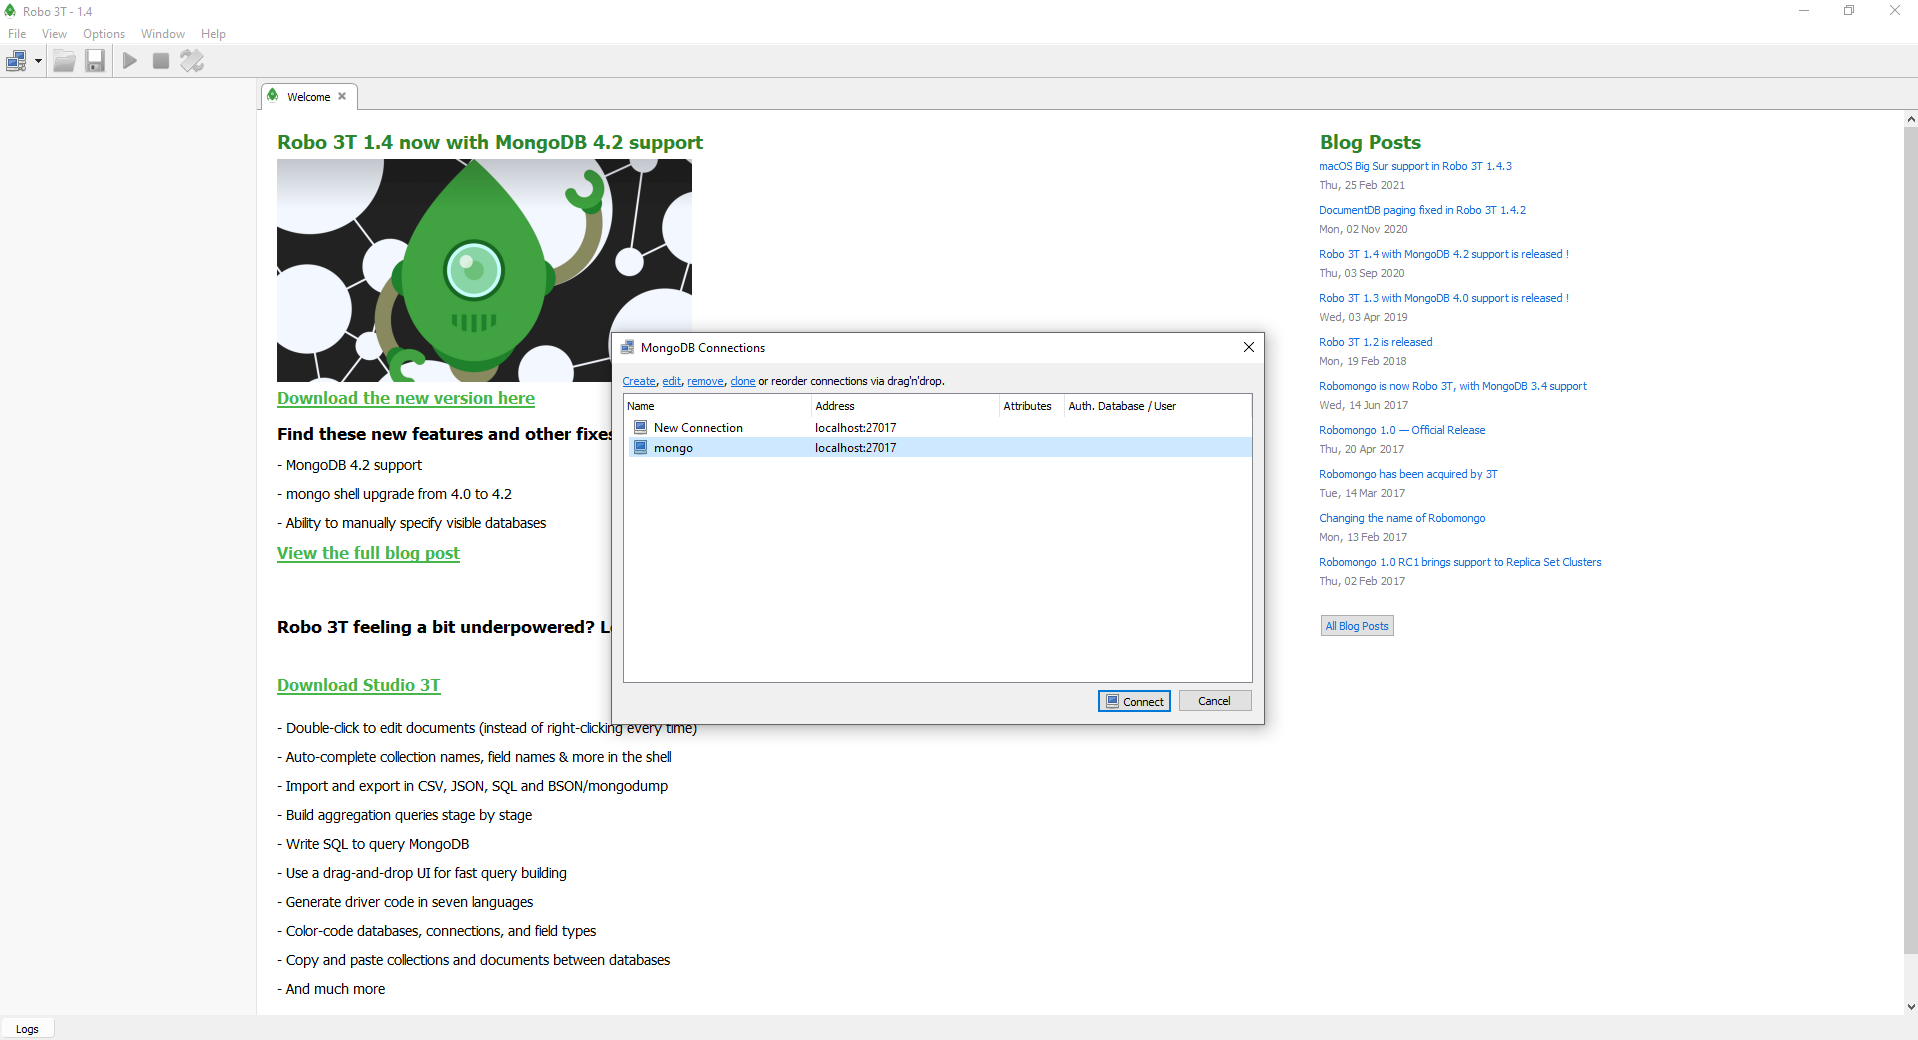
\includegraphics[scale=0.3]{img/robo-connect.PNG}\par
From here the user can select one of the connections, and providing that a MongoDB database is currently running on one of the machines ports, Robo 3T will connect to it displaying contents similar to the following: \par
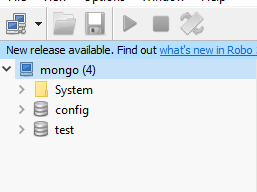
\includegraphics[]{img/robo-contents.PNG} \par
The user can then select their MongoDB database, in this case it is test, and Robo 3T will display all of the collections within this database. \par
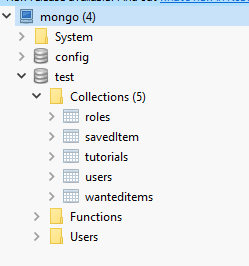
\includegraphics[]{img/robo-collections.PNG} \par
The user can then select these collections and execute various commands that would normally be entered into a command line interface. \par
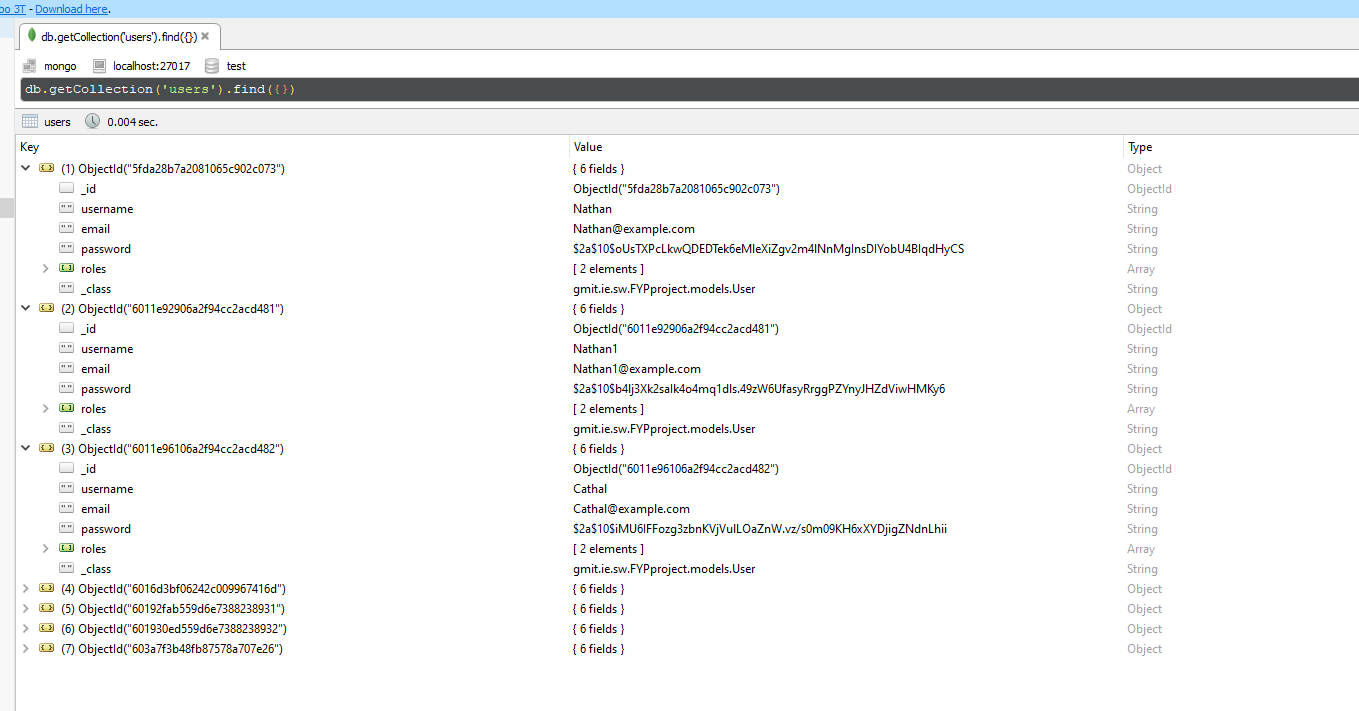
\includegraphics[scale=0.4]{img/robo-users.PNG} \newline
As we can see above, Robo 3T executes these commands, this time it being: 
\begin{minted}{console}
db.getCollection('users').find({})
\end{minted}
This can save many users the much needed time that would otherwise be lost in a CMD window trying to configure the requests and ensuring that their syntax is correct.


\subsection{Postman}

\includegraphics[scale=0.5]{img/postman-inc-logo-vector.png}
\subsection{AWS}

\includegraphics[scale = 0.4]{img/aws_logo_smile_1200x630.png}\newline
AWS, also known as Amazon Web Services, is one of the leaders in the cloud computer market. AWS was first introduced in 2002 as a means to provide tools and services to developers to incorporate features of Amazon.com into their website. Its first cloud servicing was introduced in 2006. Today, AWS offer a wide range of cloud services that span a wide array of domains. Due to this, the AWS service is now used by over 45\% of the global market. \par
AWS is a secure cloud platform that provides computing power, database, networking, content storage and much more. The platform also works on a pay-as-you-go model, meaning you only pay as long as your service is running. Some of the other advantages of AWS are:
\begin{itemize}
    \item Security: AWS provides a secure and durable platform that offers end-to-end privacy and security.
    \item Flexible: It allows users to select the OS, Language and Database and other services.
    \item Scalable: Depending on user requirements, application can be scaled up or down.
\end{itemize}
In our project, we use AWS to host the Back End environment, the Front End Environment and the MongoDB Database off of the Docker containers we built. This allowed us to host our website with ease and to deploy it in a matter of days.
\section{Development Technologies}

\subsection{IntelliJ}
This is the Integrated Development Environment that we used for our Back End Java Spring Boot API. IntelliJ has many supported features built into its system. This was the optimal IDE of choice for the Back End environment as, being wrote in Java, it is very Object Orientated based. IntelliJ analyzes the code, looking for connections between symbols across all project files and languages.\par
Using this information, it provides in depth coding assistance, quick navigation, clever error analysis and refactoring. This allows IntelliJ to auto complete many lines of code as the developer works. This is an excellent IDE for Java developers, and can save some much needed time. The smart completion ensures less errors in ones code as oppose to developing on an IDE like Eclipse. IntelliJ isn't tasking on your machine allowing for developers of all levels to create great Java code.

\subsection{Visual Studio Code}

\section{Organisation Technology}

\subsection{GitHub}

\includegraphics[scale=0.7]{img/github-logo.jpg}
GitHub has a multitude of different features to vastly improve the development of a project of any level of difficulty. GitHub is an online framework that can be used to host a variety of different programming languages such as Java, C++ and Ruby. GitHub is a git repository hosting service and can be used for version control management. \par
GitHub also has many social network functionalities built into its framework. A user on GitHub can follow other users, view their repositories and their projects, search the entirety of public GitHub repositories and more. This was the main method of storing, updating and trading code with one another. If a compile error on one of our ends were to develop, we could always clone the most recent version of our project back onto our machines instead of spending hours trying to roll back to when our own versions last compiled properly. \par
Below we will list some basic commands that users can enter into a Command-Line Interface (cmd) to initialise and to push to a repository of their own.
\subsubsection{Git commands}
\begin{minted}{console}
# to initialise a repository inside the current directory
git init

# to add all of the existing contents inside the directory to the repository
git add .

# a commit is when a user pushes to the repository. The message "first commit" can be changed to the user's preference allowing them to explain what the commit consists of
git commit -m "first commit"

# this contains the URL of the repository the user is pushing to
git remote add origin https://github.com/username/FirstRepo.git 

# command to finalise push
git push -u origin master


# push an existing repository from the command line
git add .
git commit -m "Another commit"
git push

\end{minted}

\subsection{Jira}

\subsection{Discord}

\includegraphics[scale=0.15]{img/discord-logo.jpg} \newline
The Discord application is an almost unbeatable means of communication between developers, especially in the world we live in today with the Covid-19 pandemic. Discord was essential in our development of this project, as when we were pair programming, refer to our methodology for more information on this, this was the platform we used to do so. Discord allows a user to share their screen, and all other members of the Discord call to view their screen in real time. Discord also has the feature of bots. These bots can do numerous functions. We created a Final Year Project Server on Discord for our development process. One of the bots included in this server was a bot called "Groovy". This bot allows users to enter commands into the text channels, requesting a song. The bot will automatically join the call and play the song in question. This was utilized a multitude of times to increase our moral and enthusiasm as we worked on the project. \newline
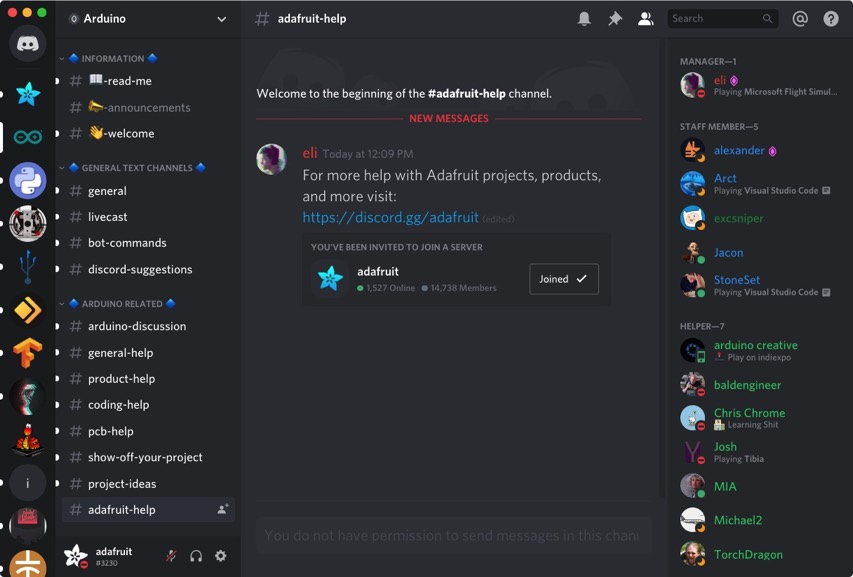
\includegraphics[scale=0.5]{img/server.jpg}
\newline

\subsection{Facebook Messenger}

\includegraphics[scale=0.3]{img/messenger.png} \newline
Facebook messenger was utilised by us as a form of communication when both of us were away from our machines. Since first year, this has been our main platform for communicating with one another so it was a natural choice for us to continue to use the platform for our planning and development. When one was working on the project and needed to get in touch with the other developer, we could utilize messenger's built in call feature. This will ring the receiver's phone the same as a normal telephone call, but doesn't require any credit, as unemployed students this was a great method for instantly getting in touch with one another.

\subsection{Microsoft Teams}

\includegraphics[scale=0.5]{img/teams-728.jpg}\newline
In 2020 when the Covid-19 restrictions first came into place in Ireland, Galway-Mayo Institute of Technology switched to the Microsoft Teams platform to continue to do live lectures and labs. As the college decided to keep our course at home for the 2 semesters of our final year, Microsoft Teams was used very often with our modules for live labs and lectures. \par
This is the platform we used to communicate with our supervisor and to meet for our weekly meetings. GMIT linked our GMIT accounts with the Microsoft office, meaning we didn't even need to create an account for ourselves, and we were already connected to all of our lecturers and fellow students, saving us some much needed time. It has vast number of different features for users. It allows the user to do most of the same functions as Discord, but we used it for a more professional manner. We had a private chat between ourselves and Martin in which we could message each other and send in photos. This was used to communicate ideas and problems we came across in the development phase. \par

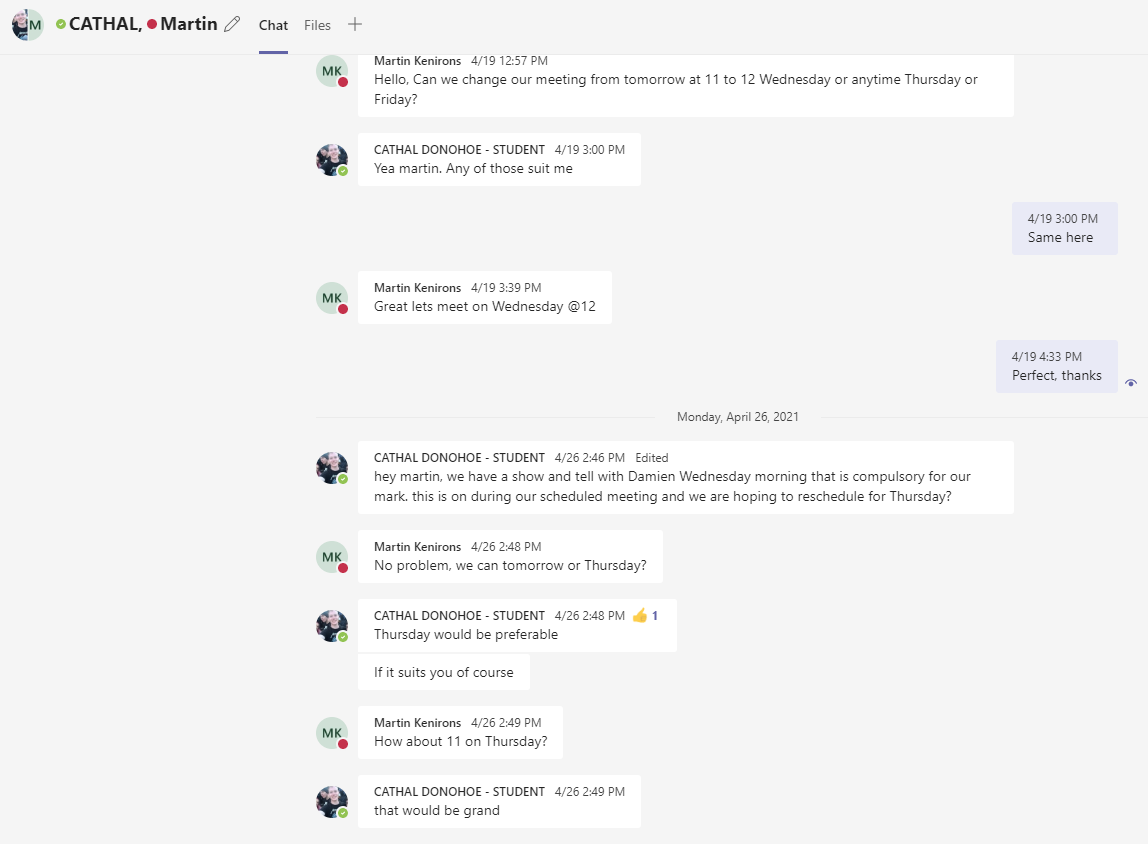
\includegraphics[scale=0.4]{img/teams.PNG}\newline
Another important feature of Microsoft Teams is the ability to schedule meetings between multiple users for a specific Date and Time. This notifies all users invited that they have a scheduled meeting for this Time and Date. This was important in keeping us on top of our weekly meetings. As i stated above with the GMIT accounts and the Microsoft accounts being linked, if we logged into Windows built in Mail application with our GMIT accounts, the scheduled meetings automatically appear on the Windows calendar, further notifying the user of a meeting and ensuring ease of use and punctuality for that user.\newline
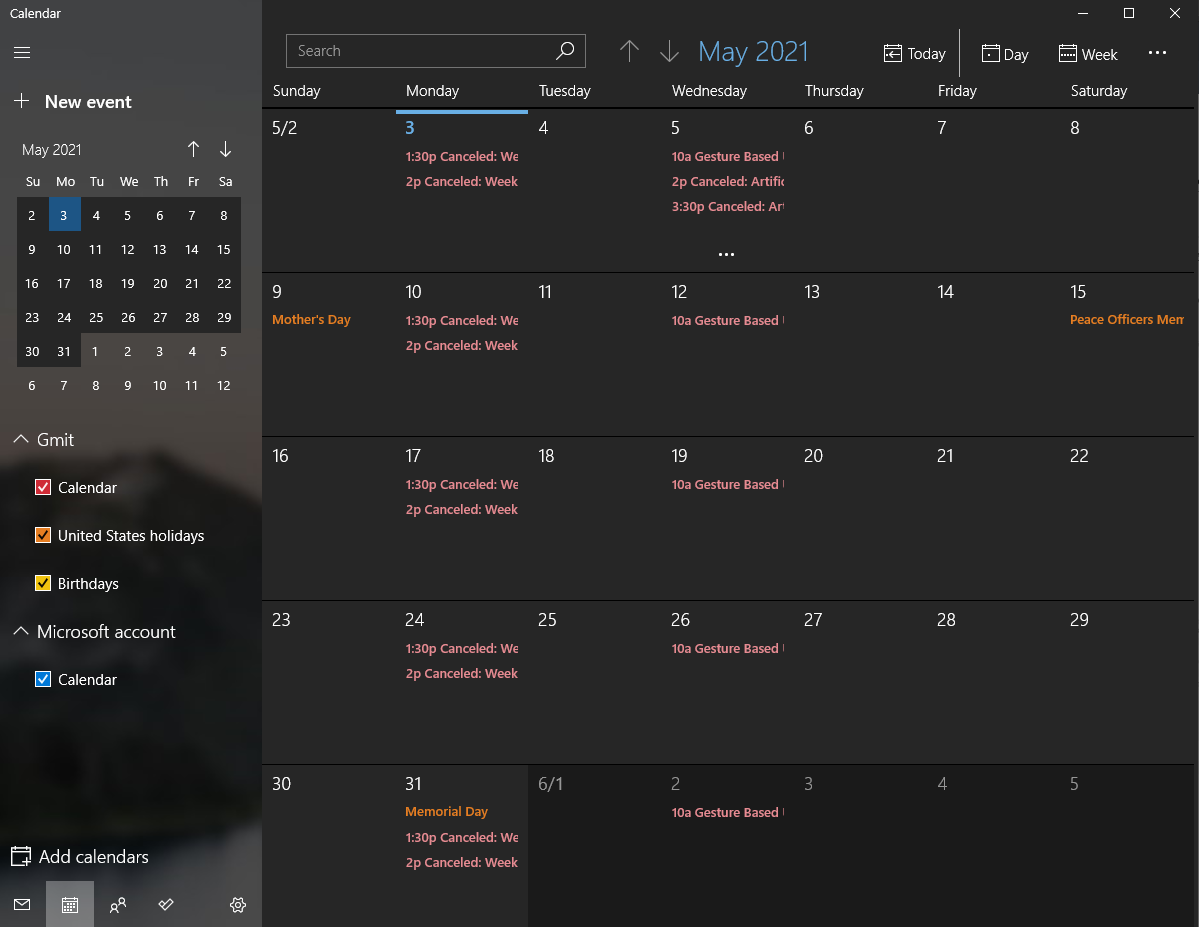
\includegraphics[scale=0.4]{img/Caledar.PNG} \newline
In teams scheduled meetings \newline
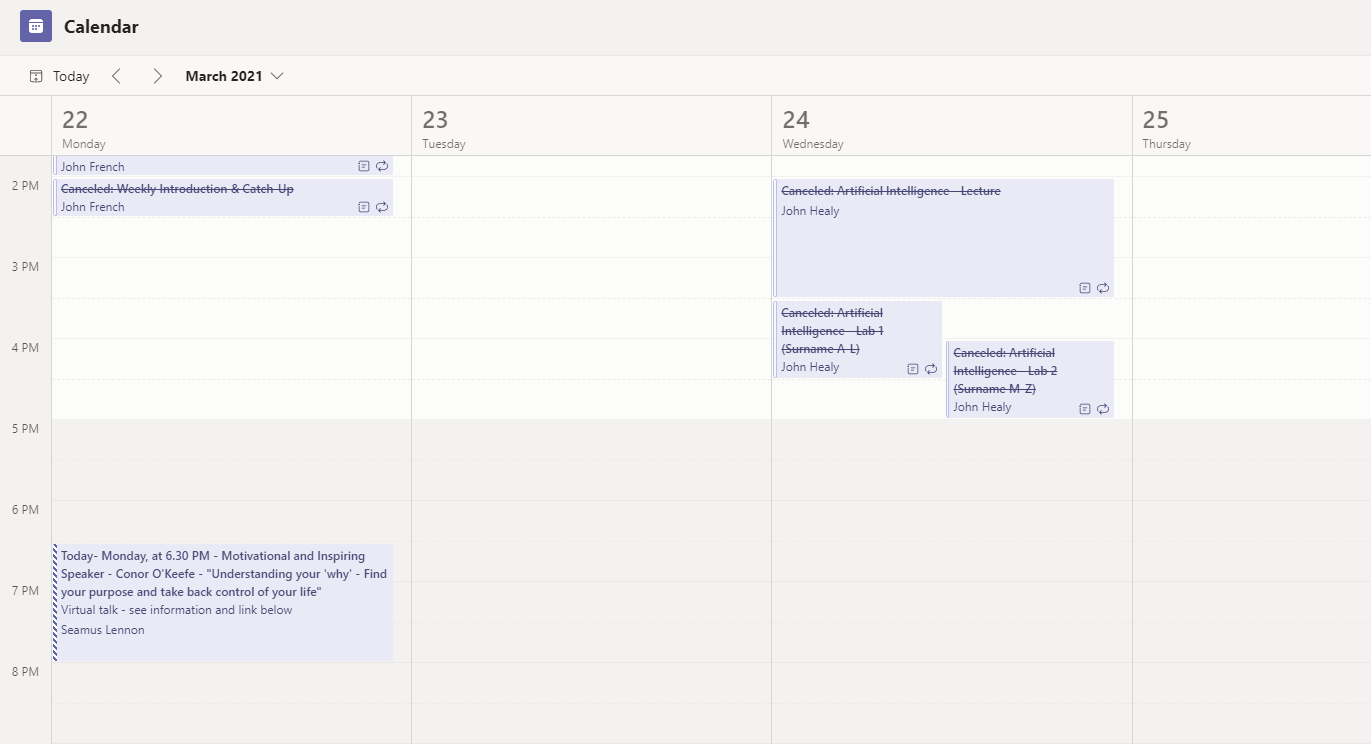
\includegraphics[scale=0.4]{img/TCalendar.PNG}\newline

\chapter{System Design}
Provide a detailed explanation of the overall system
architecture. The HOW of the project.
– System designed should be informed by the technology review, i.e.
you applied the knowledge that you learned doing the research…
– Standards-based where possible. How are components coupled?
– Cloud hosted – IaaS / PaaS / SaaS.
q Use diagrams to augment an explanation of the architecture
used.
– Provide a comprehensive overview of the different components of
the system and how they work together.
– UML class, sequence and interaction diagrams.
– Course and fine grain.
– Use screen shots of forms or other UI components.
q Page count range difficult to state as varies significantly
between projects.
As many pages as needed.
\begin{itemize}
\item Architecture, UML etc. An overview of the different components of the system. Diagrams etc… Screen shots etc.
\end{itemize}

\begin{table}[h]
  \centering
  \begin{tabular}{x{2cm}p{3cm}}
    \toprule \\
    Column 1 & Column 2 \\
    \midrule \\
    Rows 2.1 & Row 2.2 \\
    \bottomrule
  \end{tabular}
  \caption{A table.}
  \label{table:mytable}
\end{table}


\chapter{System Evaluation}
Evaluate your project against the objective set out in the
introduction.
– Prove that your software is robust. How?
• Unit / acceptance testing for robustness / behaviour.
• Stability metrics for structure.
– Any tables / graphs of results belong here.
• Provide an accompanying discussion.
– Use performance benchmarks (space and time) if algorithmic.
– Measure the outcomes / outputs of your system / software against
the objectives from the Introduction.
q Highlight any limitations or opportunities in your approach or
technologies used.
– Identifying limitations is not a sign of weakness. It is proof of
insight.
As many pages as needed.
\begin{itemize}
\item Prove that your software is robust. How? Testing etc. 
\item Use performance benchmarks (space and time) if algorithmic.
\item Measure the outcomes / outputs of your system / software against the objectives from the Introduction.
\item Highlight any limitations or opportuni-ties in your approach or technologies used.
\end{itemize}

\chapter{Conclusion}
About three pages.

\begin{itemize}
Briefly summarise your context and objectives.
– Remind the reader about the overall rationale and goals of the
project.
q Highlight your findings from the System Evaluation chapter.
– List out the outcomes of the project in a bulleted list.
– Serendipity – did you gain any tangential or even unrelated insights
by happenchance during the project?
• Lots of discoveries have been made this way, e.g. Flemming
and antibiotics.
– State any opportunities identified for future investigation.
q Finish on an upbeat note.
\item Briefly summarise your context and ob-jectives (a few lines).
\item Highlight your findings from the evalua-tion section / chapter and any opportuni-ties identified.
\end{itemize}
